\part{Betinget Optimering}

\chapter{Introduksjon til Betinget Optimering}

Betinget optimering er en sentral del av optimeringsteori som handler om å finne optimale verdier for en funksjon når variablene må tilfredsstille spesifikke betingelser eller begrensninger.

\section{Problemformulering}

Et generelt betinget optimeringsproblem kan formuleres som:
\begin{mini*}
	{x \in \mathbb{R}^n}{f(x)}{}{}
	\addConstraint{g_i(x)}{\leq 0,\quad}{ i = 1,\ldots,m}
	\addConstraint{h_j(x)}{= 0,\quad}{ j = 1,\ldots,p}
\end{mini*}

hvor:
\begin{itemize}
	\item $f(x)$ er målfunksjonen vi ønsker å minimere
	\item $g_i(x)$ er ulikhetsbetingelser som definerer tillatte øvre grenser
	\item $h_j(x)$ er likhetsbetingelser som må tilfredsstilles eksakt
\end{itemize}

Disse betingelsene definerer sammen et tillatt område (feasible region) som løsningen må ligge innenfor.

\section{Feasible Region og Retning}


\section{Lineært Betinget Optimeringsproblem}

\begin{definition}{Lineært optimeringsproblem}{linear_programming}
	Et lineært optimeringsproblem er et optimeringsproblem på formen
	\begin{mini*}
		{x\in\R^n}{c^Tx}{}{}
		\addConstraint{Ax}{\leq b,}{}
		\addConstraint{Dx}{= e,}{}
	\end{mini*}
	hvor \(c \in \R^n\) er en kostnadsvektor, \(A \in \R^{m \times n}\) er en matrise med ulikhetsbetingelser, \(D \in \R^{p \times n}\) er en matrise med likhetsbetingelser, og \(b \in \R^m\) og \(e \in \R^p\) er vektorer med høyre sideverdier.
\end{definition}

\begin{example}{Lineær funksjon}{linear_function}
	La \(f(\symbf{x}) = c^T\symbf{x} + d\) være en lineær funksjon, hvor \(c\) er en vektor normal til en hyperplan og \(d\) er en konstant.
	Da er \(f(\symbf{x}) = 0\) en lineær likning som definerer en hyperplan i \(\R^n\).
\end{example}

\begin{example}{Lineær regresjon}{linear_regression}
	La \(X \in \R^{n \times m}\) være en matrise med observasjoner og \(y \in \R^n\) være en vektor med målinger.
	Lineær regresjon er et eksempel på et lineært program hvor vi ønsker å finne en vektor \(w \in \R^m\) som minimerer kvadratfeilen
	\begin{equation*}
		\min_{w \in \R^m} \norm{Xw - y}_2^2.
	\end{equation*}
\end{example}

\section{Løsningsmetoder}

Vi skal se på ulike metoder for å løse betingede optimeringsproblemer, inkludert:
\begin{itemize}
	\item Lagranges multiplikatormetode for likhetsbetingelser
	\item KKT-betingelser for både likhets- og ulikhetsbetingelser
	\item Konveks optimering som en viktig spesialklasse
\end{itemize}


\chapter{Constraint Qualifications}

For å sikre at optimalitetsbetingelsene er gyldige og at vi kan finne Lagrange-multiplikatorer, trenger vi visse betingelser kjent som "constraint qualifications".

\section[Slaters betingelse]{\gls{slater-condition}}

\begin{definition}[breakable]{Slaters betingelse}{slater_condition}
	For et konvekst problem med ulikhetsbetingelser
	\[
		c_i(x) \le 0,\quad i=1,2,\dots,m,
	\]
	er Slaters betingelse oppfylt dersom det finnes et \(x\) slik at
	\[
		c_i(x) < 0 \quad \text{for alle } i.
	\]
\end{definition}

\begin{remark}{Intuisjon}{}
	Denne betingelsen garanterer at det tillatte området har et ikke-tomt indre.

	Med andre ord: Betingelsene er ikke alle \enquote{stramme} i hvert punkt, noe som sikrer sterk dualitet og eksistens av Lagrange-multiplikatorer.
\end{remark}

\section{Lineær Uavhengighetsbetingelse (LICQ)}
\label{sec:LICQ}

Et ikke-lineært optimeringsproblem kan skrives på følgende måte\cite[Kapittel~12]{NocedalWright2006}:
\begin{mini*}
	{x \in \mathbb{R}^n}{f(x)}{}{}
	\addConstraint{c_i(x)}{= 0,\quad}{ i \in \mathcal{E}}
	\addConstraint{c_j(x)}{\leq 0,\quad}{ j \in \mathcal{I}}
\end{mini*}

Hvor \(f : \mathbb{R}^n \to \mathbb{R}\) er den vanlige objektfunksjonen vår, men hvor \(c_i(x)\), \(c_j(x)\) representerer henholdsvis likhets- og ulikhetsbetingelser (kravene til løsningsrommet vårt \(\Omega\)).

\subsection{Definisjon av LICQ}

\begin{definition}{Linear Independence Constraint Qualification (LICQ)}{licq}
	La $x^*$ være et \emph{feasibelt} punkt. Definer mengden av aktive betingelser
	\[
		\mathcal{A}(x^*) \;=\; \{\; i \in \mathcal{E} \cup \mathcal{I} \;\mid\; c_i(x^*) = 0 \}.
	\]
	LICQ er oppfylt ved $x^*$ hvis gradientene til de aktive betingelsene
	\[
		\{\nabla c_i(x^*) :\, i \in \mathcal{A}(x^*)\}
	\]
	er lineært uavhengige i $\mathbb{R}^n$. Formelt betyr dette:
	\[
		\sum_{i \,\in\, \mathcal{A}(x^*)} \lambda_i \,\nabla c_i(x^*) \;=\; 0
		\quad \Longrightarrow \quad
		\lambda_i = 0 \;\;\text{for alle}\; i \in \mathcal{A}(x^*).
	\]
\end{definition}

\begin{remark}{Betydning av LICQ}{}
	LICQ sikrer at standard Karush--Kuhn--Tucker-(KKT)-teori er anvendelig, blant annet fordi:
	\begin{itemize}
		\item Eventuelle Lagrange-multiplikatorkoordinater (for de aktive betingelsene) er veldefinerte
		\item Disse multiplikatorene er ofte unike
		\item KKT-betingelsene blir nødvendige optimalitetsbetingelser
	\end{itemize}
\end{remark}

\subsection{Rollen til LICQ i KKT-teori}

Følgende punkter fremhever hvorfor LICQ er sentralt:
\begin{enumerate}
	\item \textbf{Eksistens av Lagrange-multiplierne:} Hvis \(x^*\) er et lokalt minimum og LICQ gjelder ved \(x^*\), eksisterer en unik vektor \(\lambda^*\) av multiplikatorer for de aktive betingelsene slik at KKT-betingelsene
	      \[
		      \nabla f(x^*) \;=\; \sum_{i \,\in\, \mathcal{A}(x^*)}\!\lambda_i^*\,\nabla c_i(x^*),\quad
		      \lambda_j^* \,\ge\,0 \text{ for aktive ulikheter},
	      \]
	      samt komplementaritetsbetingelser, blir oppfylt.
	\item \textbf{Lokal regularitet:} Dersom LICQ holder, har Jakobi-matrisen for de aktive betingelsene full rang.
	      Dette sikrer at gradientene til de aktive betingelsene er lineært uavhengige, noe som er nødvendig for å kunne bruke KKT-betingelsene.
	\item \textbf{Unikhet av multiplikatorer:} Hvis LICQ er oppfylt, er multiplikatorene entydige. Dette betyr at det ikke finnes flere løsninger for multiplikatorene som tilfredsstiller KKT-betingelsene.
\end{enumerate}
Hvis LICQ ikke holder, kan det oppstå problemer med å finne Lagrange-multiplikatorene, og KKT-betingelsene kan bli ugyldige eller gi flere løsninger.
\begin{example}{LICQ med flere ulikhetsbetingelser}{}
	La oss se på følgende optimeringsproblem med diverse ulikhetsbetingelser:
	\begin{mini*}
		{x,y}{(x-1)^2 + (y+2)^2}{}{}
		\addConstraint{c_1(x,y) &= -x}{\leq 0}{}
		\addConstraint{c_2(x,y) &= x-2-y}{\leq 0}{}
		\addConstraint{c_3(x,y) &= 1-(x-1)^2-y^2}{\leq 0}{}
	\end{mini*}

	Ved punkt \(P\) hvor alle tre betingelser møtes, har vi følgende gradienter:
	\begin{align*}
		\nabla c_1(x,y) & = (-1,0),        \\
		\nabla c_2(x,y) & = (1,-1),        \\
		\nabla c_3(x,y) & = (-2(x-1),-2y).
	\end{align*}

	% Taken from: TMA4180 - Optimization 1 - NTNU 
% Exam Autumn 2024 - Problem 2

\documentclass[tikz,border=5pt]{standalone}
\usepackage{tikz}

\begin{document}

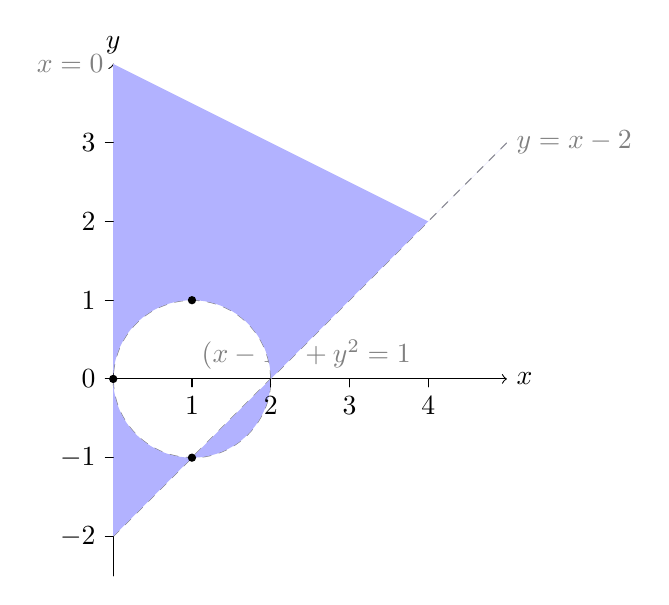
\begin{tikzpicture}[scale=1, line cap=round, line join=round]

  \draw[->] (-0.1,0) -- (5,0) node[right] {\(x\)};
  \draw[->] (0,-2.5) -- (0,4) node[above] {\(y\)};
  
  % Feasible region: outside the circle, with x ≥ 0 and y ≥ x − 2
  \draw[dashed, color=gray] (0,-2) -- (5,3) node[right]{\(y=x-2\)};
  \draw[dashed, color=gray] (0,-2) -- (0,4) node[left]{\(x=0\)};
  \draw[dashed, color=gray] (1,0) circle (1) node[above right]{\((x-1)^2+y^2=1\)};
  \node at (1,2) {\(\Omega\)};
  \fill[blue!30, even odd rule] 
    (0,-2) -- (5,3) -- (4,2) -- (0,4) -- cycle
    (1,0) circle (1);
    
  \foreach \x in {1,2,3,4}{
    \draw (\x,0) -- (\x,-0.1) node[below] {\(\x\)};
  }

  \foreach \y in {-2,-1,0,1,2,3}{
    \draw (0,\y) -- (-0.1,\y) node[left] {\(\y\)};
  }

  \fill (1,1)   circle(1.5pt);
  \fill (0,0)   circle(1.5pt);
  \fill (1,-1) circle(1.5pt);



\end{tikzpicture}

\end{document}


	Ved punkt \(P\) hvor alle tre betingelser møtes, kan vi se at gradientene peker i forskjellige retninger og er lineært uavhengige. Derfor er LICQ oppfylt ved dette punktet.

	Dette er viktig for å kunne bruke KKT-betingelsene til å finne den optimale løsningen.

\end{example}


\begin{remark}{LICQ -- Kort Fortalt}
	LICQ består av to nøkkelelementer:
	\paragraph{Aktive betingelser} En betingelse er aktiv hvis:
	\[ \begin{cases}
			c_i(\symbf{x}) = 0 & \text{for likhetsbetingelser}         \\
			c_j(\symbf{x}) = 0 & \text{for aktive ulikhetsbetingelser}
		\end{cases} \]
	\paragraph{Lineær uavhengighet} Gradientene \(\{\nabla c_k(\symbf{x}^\star)\}\) til de aktive betingelsene må være lineært uavhengige, altså:
	\[
		\sum_k \alpha_k \nabla c_k(\symbf{x}^\star) = 0 \implies \alpha_k = 0 \text{ for alle } k
	\]
\end{remark}

\subsection{Oppsummering}

Lineær Uavhengighetsbetingelse (LICQ) er en kjernenødvendighet for mange algoritmer og analytiske metoder innen ikke-lineær optimering. Den sikrer at de aktive betingelsene ved et punkt \(x^*\) er ``pent'' ordnet, i den forstand at ingen av gradientene er lineært avhengige. Når LICQ er gyldig, kan man utlede KKT-betingelsene og ofte fastslå entydige multiplikatorer. Som eksempel viser vi at betingelser som er multiple av hverandre (redundante) fører til brudd på LICQ og kan komplisere både teori og numeriske metoder.

\chapter{Optimalitetsbetingelser}

\section{Lagrangian-funksjonen}
\begin{definition}{The Lagrangian of a problem}{lagrangian}
	The Lagrangian of a problem is the function \(\mathcal{L}: \mathbb{R}^d \times \mathbb{R}^m \times \mathbb{R}^l \times \mathbb{R}^e \to \mathbb{R}\) defined as:
	\begin{align*}
		\mathcal{L}(x, \lambda, \mu, v) & = f(x) + \sum_{i\in \mathcal{I}} \lambda_i c_i(x) + \sum_{1 \leq i \leq m} \mu_i (Ax - b)_i + \sum_{1 \leq i \leq l} v_i (Cx - b)_i                               \\
		                                & = f(x) - \sum_{i \in \mathcal{I}} \lambda_i c_i(x) - \inner{\mu, Ax - b} - \inner{v, Cx - e}\footnote{\( (1) \iff \nabla_x \mathcal{L}(x, \lambda, \mu, v) = 0\)}
	\end{align*}
\end{definition}

Lagrangian-funksjonen gjør det mulig å håndtere betingelser ved å innføre multiplikatorer som vekter viktigheten av hver betingelse. Dette omformer et betinget optimeringsproblem til et ubetinget problem der vi søker sadelpunkter for Lagrangian-funksjonen.

\section{Farkas' lemma}

\begin{lemma}{Farka's Lemma}{farkas_lemma}
	Let \(A \in \mathbb{R}^{m \times n}\) and \(c \in \mathbb{R}^n\). Then, exactly one of the following statements is true:
	\begin{enumerate}
		\item[] \((1)\) There exists an \(x \in \mathbb{R}^n\) such that \(Ax \preceq 0\) and \(c^T x < 0\).
		\item[] \((2)\) There exists a \(y \in \mathbb{R}^m\) such that \(A^T y + c = 0\) and \(y \succeq 0\).
	\end{enumerate}
\end{lemma}

\begin{proof}
	\begin{enumerate}
		\item[] Assume that \((1)\) holds. Then \(Ax = b\) and \(x \ge 0\). If there exists a \(y\) such that \(y^T A \ge 0\), then
		      \[
			      y^T b = y^T Ax = (y^T A)x \ge 0,
		      \]
		      which contradicts \(y^T b < 0\).
		\item[] Assume that \((1)\) does not hold. We want to show that \((2)\) holds.

		      Let
		      \[
			      K = \{Ax \mid x \ge 0\}.
		      \]
		      Since \((1)\) does not hold, \(b \notin K\). Since \(K\) is a closed convex cone, by the separating hyperplane theorem, there exists a \(y \in \mathbb{R}^m\) such that
		      \[
			      y^T b < y^T z \quad \text{for all } z \in K.
		      \]
		      Since \(0 \in K\), we have \(y^T b < 0\).

		      Now, for any \(x \ge 0\), we have \(Ax \in K\), so \(y^T b < y^T Ax\).

		      Let \(x = e_i\), where \(e_i\) is the \(i\)-th standard basis vector. Then \(x \ge 0\), and
		      \[
			      y^T A e_i = (y^T A)_i > 0.
		      \]
		      Thus \(y^T A \ge 0\).
	\end{enumerate}

	\begin{center}
		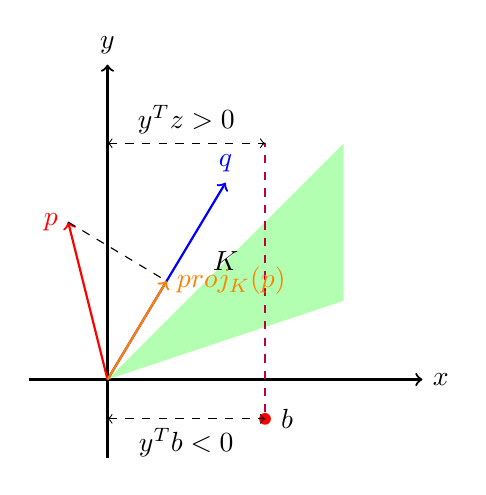
\begin{tikzpicture}
			\draw[->, thick] (-1, 0) -- (4, 0) node[right] {$x$};
			\draw[->, thick] (0, -1) -- (0, 4) node[above] {$y$};

			\fill[green!30] (0, 0) -- (3, 1) -- (3, 3) -- cycle;
			\node at (1.5, 1.5) {$K$};

			\node[circle, fill=red, inner sep=1.5pt, label=right:$b$] (b) at (2, -0.5) {};

			\draw[dashed, purple] (b) -- (2, 3);
			\draw[<->, dashed, black] (0, -0.5) -- (2, -0.5) node[midway, below, black] {$y^Tb < 0$};
			\draw[<->, dashed, black] (0, 3) -- (2, 3) node[midway, above, black] {$y^Tz > 0$};

			% Adding new vectors
			\draw[->, thick, blue] (0, 0) -- (1.5, 2.5) node[above] {$q$};
			\draw[->, thick, red] (0, 0) -- (-0.5, 2) node[left] {$p$};
			\draw[->, thick, orange] (0, 0) -- (0.75, 1.25) node[right] {$proj_K(p)$};
			\draw[dashed] (-0.5, 2) -- (0.75, 1.25);
		\end{tikzpicture}
	\end{center}

	The figure illustrates the geometric interpretation of Farkas' Lemma. The green region $K$ represents the cone of feasible points $\{Ax \mid x \ge 0\}$. The point $b$ (in red) lies outside this cone. The purple dashed line represents the separating hyperplane, which separates $b$ from $K$. Vector $p$ (in red) is projected onto the cone $K$, resulting in $proj_K(p)$ (in orange). Vector $q$ (in blue) lies inside the cone $K$. The black dashed lines show that the inner product $y^Tb$ is negative, while the inner product $y^Tz$ is positive for points $z$ in the cone $K$.
\end{proof}

\section[KKT-betingelser]{\gls{kkt-conditions}}

\begin{theorem}{KKT conditions}{kkt}
	\begin{align*}
		\mathcal{A}_1(x)            & := \{i \in \mathcal{I} \mid c_i(x) = 0\},                     \\
		\mathcal{A}_2(x)            & := \{1 \leq i \leq m \mid (Ax)_i = b_i\} \tag{Active indices} \\
		\text{Active indices at } x & \in \Omega                                                    \\
	\end{align*}

	\begin{itemize}
		\item \(A_i\) are the active constraints/indices at \(x\)
		\item \(C\) is the matrix of equality constraints.
		\item \(p\) is the direction of descent.
		\item \(x\) is the current point (feasible).
		\item \(T_{\Omega}(x)\) is the tangent cone at \(x\).
		\item \(c_i(x)\) is the value of the \(i\)-th constraint at \(x\).
		\item \(Ax\) is the value of the equality constraints at \(x\).
		\item \(b\) is the vector of equality constraints.
	\end{itemize}

	Assume that \emph{Slater's constraint} holds. Then, the following statements are equivalent:

	\begin{align*}
		p\in T_{\Omega}(x) & \Longleftrightarrow
		\begin{cases}
			\inner{\nabla c_i(x), p} \geq 0, & i \in \mathcal{A}_1(x) \\
			(Ax)_i \geq 0,                   & i \in \mathcal{A}_2(x) \\
			Cp = 0,                          &                        \\
		\end{cases}
	\end{align*}
\end{theorem}

\begin{theorem}{KKT conditions}{kkt_conditions}
	Assume \(c_i, i \in \mathcal{I}\) are concave in \(\mathcal{C}^1\),
	\(A\in \mathbb{R}^{m \times d}, b \in \mathbb{R}^m\) and \(C\in \mathbb{R}^{l \times d}\) and that \(f:\mathbb{R}^d \to \mathbb{R}\) is \(\mathcal{C}^1\). Assume that \emph{Slater's condition} holds.

	If \(x^\star\) is a local minimum of \(\min_x f(x)\) s.t.
	\[
		\begin{cases}
			c_i(x) \geq 0, & \forall i \in \mathcal{I} \\
			Ax \geq b,     &                           \\
			Cx = b,        &
		\end{cases}
	\]
	then there exists a \emph{Lagrange multipliers} \(\lambda^\star, \mu^\star\) with \(v \in \R^e\) s.t. the \emph{KKT conditions} hold:

	Then, the following statements are equivalent:
	\begin{align}
		\nabla f(x^\star) = \sum_{i\in \mathcal{I}} \lambda_i^\star \nabla c_i(x^\star) + A^T \mu^\star + C^T v^\star \\
		\begin{cases}
			c_i(x^\star) \geq 0, & \forall i \in \mathcal{I} \\
			Ax^\star \geq b,     &                           \\
			Cx^\star = e,        &                           \\
		\end{cases} \tag{Feasibility}                                                              \\
		\begin{cases}
			\lambda_i^\star \geq 0, & \forall i \in \mathcal{I} \\
			\mu_j^\star \in \geq 0, & \forall j \in \mathcal{J} \\
		\end{cases} \tag{Dual feasibility}                                                           \\
		\begin{cases}
			\lambda_i^\star c_i(x^\star) = 0, & \forall i \in \mathcal{I} \\
			\mu_j^\star C_j^T = 0,            & \forall j \in \mathcal{J} \\
		\end{cases} \tag{Complementary slackness}                                                 \\
		\begin{cases}
			\lambda_i^\star c_i(x^\star) = 0,      & \forall i \in \mathcal{I} \\
			\inner{\mu_j^\star, Ax^\star - b} = 0, & \forall j \in \mathcal{J} \\
		\end{cases} \tag{Complementary slackness}
	\end{align}
\end{theorem}

\begin{proof}{}{}
	We have the optimality condition:
	\[
		\inner{\nabla f(x^\star), p} \geq 0 \, \forall p \in T_{\Omega}(x^\star)
	\]
	\medskip
	\begin{align*}
		p \in T_{\Omega}(x^\star) \iff
		\begin{cases}
			\inner{\nabla c_i (x^\star), p }\geq 0                             & \forall i \in \mathcal{A}_1(x^\star) \\
			\text{or: there does not exist any } p \in \R^d \text{ such that:} &                                      \\
			\begin{cases}
				\inner{\nabla c_i (x^\star), p }\geq 0 & \forall i \in \mathcal{A}_1(x^\star) \\
				\inner{A_i^T , p }\geq 0               & \forall i \in \mathcal{A}_2(x^\star) \\
				\inner{ (C_i )^T, p } = 0              & \forall 1 \leq i \leq l              \\
				\inner{\nabla f (x^\star), p } < 0     &
			\end{cases}                             \\
			(Ap)_i \geq 0                                                      & \forall i \in \mathcal{A}_2(x^\star) \\
			Cp = 0                                                             &
		\end{cases}
	\end{align*}

	The second alternative is Farka's Lemma does not hold \(\implies\) The first holds.

	\begin{align*}
		\nabla f(x^\star) & = \sum_{i\in \mathcal{A}_1(x^\star)} \lambda_i^\star \nabla c_i(x^\star) + \sum_{i \in \mathcal{A}_2(x^\star)} \mu_i^\star A_i^T + \sum_{i=1}^l v_i^\star C_i^T \\
	\end{align*}

	For some  \(\lambda_i^\star \geq 0, \mu_i^\star \geq 0, v_i^\star \in \R\).

	Now define: \(\lambda_i^\star = 0 \) for \(i \notin \mathcal{A}_1(x^\star)\) and \(\mu_i^\star = 0\) for \(i \notin \mathcal{A}_2(x^\star)\).

	Then we have:
	\begin{align*}
		\nabla f(x^\star) & = \sum_{i\in \mathcal{I}} \lambda_i^\star \nabla c_i(x^\star) + \sum_{1 \leq i \leq m} \mu_i^\star A_i^T + \sum_{1 \leq i \leq l} v_i^\star C_i^T = \text{(1)} \\
	\end{align*}
	\qed
\end{proof}

\section{Geometrisk tolkning av KKT-betingelsene}

KKT-betingelsene har en klar geometrisk tolkning som er nyttig for å forstå deres betydning:

\begin{itemize}
	\item \textbf{Stasjonæritetsbetingelsen} (gradienten av Lagrangian er null) betyr at gradienten til målfunksjonen kan uttrykkes som en lineær kombinasjon av gradientene til de aktive betingelsene.
	\item \textbf{Primal feasibility} sikrer at løsningen tilfredsstiller alle opprinnelige betingelser.
	\item \textbf{Dual feasibility} (multiplikatorene for ulikheter er ikke-negative) sikrer at vi beveger oss i riktig retning langs betingelsene.
	\item \textbf{Komplementaritetsbetingelsen} forteller at en betingelse enten må være aktiv (likhet), eller så må den tilhørende multiplikatoren være null.
\end{itemize}

Denne geometriske tolkningen hjelper oss å visualisere hvordan KKT-betingelsene karakteriserer optimale punkter i et betinget optimeringsproblem.

\chapter{Konveks optimering}

\section{Egenskaper ved konvekse problemer}

Hvis et optimeringsproblem er konvekst, kan vi være sikre på at vi finner en global optimal løsning. Et konvekst optimeringsproblem har følgende egenskaper:
\begin{itemize}
	\item Målfunksjonen $f$ er konveks
	\item Likhetsbetingelsene $h_j$ er lineære (affine)
	\item Ulikhetsbetingelsene $g_i$ er konvekse
\end{itemize}

Konvekse optimeringsproblemer har flere fordelaktige egenskaper:
\begin{itemize}
	\item Ethvert lokalt minimum er også et globalt minimum
	\item KKT-betingelsene er både nødvendige og tilstrekkelige for optimalitet
	\item Det finnes effektive algoritmer for å løse konvekse problemer
\end{itemize}

\section{Dualitet i konveks optimering}

For konvekse optimeringsproblemer kan vi definere et dualt problem som gir en nedre grense på verdien av det primale problemet. Under visse betingelser, som Slaters betingelse, vil det primale og duale problemet ha samme optimale verdi - dette kalles "sterk dualitet".

Dualitetsteori gir oss viktige innsikter om optimale løsninger og multiplikatorer, og danner grunnlaget for mange effektive algoritmer for konveks optimering.

\begin{center}
	\begin{tikzpicture}[
			node distance=0.8cm and 0.8cm,
			every node/.style={draw, rectangle, rounded corners=3pt, align=center, font=\sffamily\scriptsize},
			>=stealth, thick,
			startstop/.style={rectangle, rounded corners, draw, fill=cor-color!15, text width=9em, minimum height=1em},
			block/.style={rectangle, draw, fill=thm-color!10, text width=10em, rounded corners, minimum height=1em},
			decision/.style={diamond, draw, fill=lem-color!10, text width=5em, text badly centered, inner sep=0pt, aspect=1.5}
		]

		% Top-level problem
		\node [startstop] (start) {
			\textbf{Betinget Optimeringsproblem}\\[0.5ex]
			Minimer $f(x)$ gitt\\
			$c_i(x)=0,\;i\in E$;\\
			$c_j(x)\ge0,\;j\in I$
		};

		% Decision: convex?
		\node [decision, below=1.0cm of start] (convexq) {
			Er problemet\\
			\emph{konvekst}?
		};

		% --- Convex branch (left) ---
		\node [block, below left=1.0cm and 2cm of convexq] (slater) {
			\textbf{Sjekk Slaters Betingelse}\\[0.5ex]
			(for konvekse problemer)\\
			Sikrer sterk dualitet \& KKT gyldighet
		};

		\node [decision, below=1.0cm of slater] (cqok2) {
			Slater\\oppfylt?
		};

		\node [block, below=1.0cm of cqok2] (cqsat2) {
			\textbf{Slater's Betingelse:}\\[0.5ex]
			Eksisterer et punkt $\bar{x}$ der\\
			$c_j(\bar{x}) > 0$ for $j \in I$,\\
			$c_i(\bar{x}) = 0$ for $i \in E$,\\
			og $c_j(\bar{x})$ er \emph{strikt} positiv
		};

		% --- Nonconvex branch (right) ---
		\node [block, below right=1.0cm and 2cm of convexq] (licq) {
			\textbf{Sjekk KK for ikke-konvekse:}\\[0.5ex]
			\textbf{LICQ} eller MFCQ, osv.\\
			Hvis ikke oppfylt, KKT gjelder kanskje ikke
		};

		\node [decision, below=1.0cm of licq] (cqok) {
			KK\\oppfylt?
		};

		\node [block, below=1.0cm of cqok] (cqsat) {
			\textbf{LICQ:}\\[0.5ex]
			Eksisterer et punkt $\bar{x}$ der\\
			$c_i(\bar{x}) = 0$ for $i \in E$\\
			$c_j(\bar{x}) > 0$ for $j \in I$,\\
			og $\nabla c_i(\bar{x})$ er lineært uavhengige
		};

		% Failure node (shared by both branches)
		\node [block, below=1.0cm of convexq] (fail) {
			\textbf{Ingen KK oppfylt:}\\[0.5ex]
			KKT kan feile\\
			Bruk alternative metoder
		};

		% --- Common branch: KKT, Second-order, Conclusion ---
		\node [block, below=3.5cm of convexq] (kkt) {
			\textbf{KKT-betingelser:}\\[0.5ex]
			1. Stasjonaritet: $\nabla f(x^*) + \sum_i \lambda_i \nabla c_i(x^*) = 0$\\
			2. Primal gyldighet: $c_i(x^*) = 0$ eller $c_j(x^*) \geq 0$\\
			3. Dual gyldighet: $\lambda_j \geq 0$ for $j \in I$\\
			4. Komplementær slakkhet: $\lambda_j\,c_j(x^*) = 0$
		};

		\node [block, below=1.0cm of kkt] (second) {
			\textbf{Andregrads-betingelser:}\\[0.5ex]
			\emph{Nødvendig:} $\nabla_{xx}^2 \mathcal{L}(x^*,\lambda^*) \succeq 0$\\[0.5ex]
			\emph{Tilstrekkelig:} $\nabla_{xx}^2 \mathcal{L}(x^*,\lambda^*) \succ 0$
		};

		\node [startstop, below=1.0cm of second] (conclude) {
			\textbf{Konklusjon}\\[0.5ex]
			Hvis KKT + 2.-grads betingelser holder,\\
			$\;x^*$ er lokalt minimum.\\[0.5ex]
			Under konveksitet er $\;x^*$ globalt minimum.
		};

		% -----------------
		% Connections
		\draw [->, thick] (start) -- (convexq);
		\draw [->, thick] (convexq) -- node[above left, font=\tiny, fill=white] {Yes} (slater);
		\draw [->, thick] (convexq) -- node[above right, font=\tiny, fill=white] {No} (licq);

		% Convex branch
		\draw [->, thick] (slater) -- (cqok2);
		\draw [->, thick] (cqok2) -- node[font=\tiny, fill=white] {Yes} (cqsat2);
		\draw [->, thick] (cqok2.east) -- ++(1,0) |- node[font=\tiny, fill=white] {No} (fail.west);
		\draw [->, thick] (cqsat2.east) -- ++(0.5,0) |- (kkt.west);

		% Nonconvex branch
		\draw [->, thick] (licq) -- (cqok);
		\draw [->, thick] (cqok) -- node[font=\tiny, fill=white] {Yes} (cqsat);
		\draw [->, thick] (cqok.west) -- ++(-1,0) |- node[font=\tiny, fill=white] {No} (fail.east);
		\draw [->, thick] (cqsat.west) -- ++(-0.5,0) |- (kkt.east);

		% Common branch
		\draw [->, thick] (kkt) -- (second);
		\draw [->, thick] (second) -- (conclude);
	\end{tikzpicture}
\end{center}